In this section, we evaluate our model on the task of question answering using the recently released SQuAD~\citep{rajpurkar2016squad}, which has gained a huge attention over a few months. In the next section, we evaluate our model on the task of cloze-style reading comprehension. 


\paragraph{Dataset.}
SQuAD is a machine comprehension dataset on a large set of Wikipedia articles, with more than 100,000 questions. The answer to each question is always a span in the context. 
The model is given a credit if its answer matches one of the human written answers.  
Two metrics are used to evaluate models: Exact Match (EM) and a softer metric, F1 score, which measures the weighted average of the precision and recall rate at character level. 
The dataset consists of 90k/10k train/dev question-context tuples with a large hidden test set. 
It is one of the largest available MC datasets with human-written questions and serves as a great test bed for our model.

\paragraph{Model Details.}\label{subsec:squad-details}
The model architecture used for this task is depicted in Figure~\ref{fig:model}. Each paragraph and question are tokenized by a regular-expression-based word tokenizer (PTB Tokenizer) and fed into the model. We use 100 1D filters for CNN char embedding, each with a width of 5. 
The hidden state size ($d$) of the model is 100. 
The model has about 2.6 million parameters.
We use the AdaDelta~\citep{adadelta} optimizer, with a minibatch size of 60 and an initial learning rate of $0.5$, for 12 epochs. 
A dropout~\citep{dropout} rate of $0.2$ is used for the CNN, all LSTM layers, and the linear transformation before the softmax for the answers. 
During training, the moving averages of all weights of the model are maintained with the exponential decay rate of $0.999$. 
At test time, the moving averages instead of the raw weights are used.
The training process takes roughly 20 hours on a single Titan X GPU. We also train an ensemble model consisting of 12 training runs with the identical architecture and hyper-parameters. 
At test time, we choose the answer with the highest sum of confidence scores amongst the 12 runs for each question.

\paragraph{Results.} The results of our model and competing approaches on the hidden test  are summarized in Table~\ref{tab:squad-test}. \sysshort\ (ensemble) achieves an EM score of 73.3 and an F1 score of 81.1, outperforming all previous approaches.

\begin{table}[]
% \parbox{.45\linewidth}{
\begin{subfigure}[htbp]{0.6\textwidth}
    \centering
    \scalebox{0.9}{
    \begin{tabular}{lcccc}
        \hline
         & \multicolumn{2}{c}{Single Model} & \multicolumn{2}{c}{Ensemble} \\
         & EM & F1 & EM & F1\\
        \hline
        \hline
        Logistic Regression Baseline$^a$ & 40.4 & 51.0 & - & -\\
        %Match LSTM$^{2}$ & 60.5 & 70.7\\
        Dynamic Chunk Reader$^{b}$ & 62.5 & 71.0 & - & -\\
        Fine-Grained Gating$^c$ & 62.5 & 73.3 & - & -\\
        Match-LSTM$^{d}$ & 64.7 & 73.7 & 67.9 & 77.0\\
        Multi-Perspective Matching$^e$ & 65.5 & 75.1 & 68.2 & 77.2 \\
        Dynamic Coattention Networks$^{f}$ & 66.2 & 75.9 & 71.6 & 80.4 \\
        R-Net$^{g}$ & \textbf{68.4} & \textbf{77.5} & 72.1 & 79.7\\
        \sysshort\ (Ours) & 68.0 & 77.3 & \textbf{73.3} & \textbf{81.1} \\
        \hline
        
    \end{tabular}
    }
    \caption{Results on the SQuAD test set}
    \label{tab:squad-test}
%}
\end{subfigure}
\begin{subfigure}[htbp]{0.4\textwidth}
%\parbox{.45\linewidth}{
    \centering
    \scalebox{0.9}{
    \begin{tabular}{lcc}
        \hline
         & EM & F1\\
        \hline
        \hline
        No char embedding & 65.0 & 75.4\\
        No word embedding & 55.5 & 66.8\\
        No C2Q attention & 57.2 & 67.7 \\ 
        No Q2C attention & 63.6 & 73.7 \\
        Dynamic attention & 63.5 & 73.6\\
        \hline
        \sysshort\ (single) & 67.7 & 77.3 \\
        \sysshort\ (ensemble) & 72.6 & 80.7 \\
        \hline
    \end{tabular}
    }
    \caption{Ablations on the SQuAD dev set}
    \label{tab:squad-dev}
%}
\end{subfigure}
\caption{(\ref{tab:squad-test}) The performance of our model \sysshort\ and competing approaches by \cite{rajpurkar2016squad}$^a$, \cite{chunk}$^b$, \cite{yang2016words}$^c$, \cite{wang2016machine}$^d$, IBM Watson$^e$ (unpublished), \cite{dcn}$^f$, and Microsoft Research Asia$^g$ (unpublished) on the SQuAD test set.
A concurrent work by \cite{lee2016learning} does not report the test scores. 
All results shown here reflect the SQuAD leaderboard (\url{stanford-qa.com}) as of 6 Dec 2016, 12pm PST. 
(\ref{tab:squad-dev}) The performance of our model and its ablations on the SQuAD dev set. Ablation results are presented only for single runs.}
\end{table}

\paragraph{Ablations.} Table~\ref{tab:squad-dev} shows the performance of our model and its ablations on the SQuAD dev set. Both char-level and word-level embeddings contribute towards the model's performance. We conjecture that word-level embedding is better at representing the semantics of each word as a whole, while char-level embedding can better handle out-of-vocab (OOV) or rare words. To evaluate bi-directional attention, we remove C2Q and Q2C attentions. For ablating C2Q attention, we replace the attended question vector $\tilde{\bf U}$ with the average of the output vectors of the question's contextual embedding layer (LSTM). C2Q attention proves to be critical with a drop of more than 10 points on both metrics. For ablating Q2C attention, the output of the attention layer, ${\bf G}$, does not include terms that have the attended Q2C vectors, $\tilde{\bf H}$. To evaluate the attention flow, we study a dynamic attention model, where the attention is dynamically computed within the modeling layer's LSTM, following previous work~\citep{Bahdanau2014NeuralMT,wang2016machine}. This is in contrast with our approach, where the attention is pre-computed before flowing to the modeling layer. Despite being a simpler attention mechanism, our proposed static attention outperforms the dynamically computed attention by more than 3 points. We conjecture that separating out the attention layer results in a richer set of features computed in the first 4 layers which are then incorporated by the modeling layer.
We also show the performance of \sysshort\ with several different definitions of $\alpha$ and ${\bm \beta}$ functions (Equation~\ref{eqn:sim} and~\ref{eqn:flow}) in Appendix~\ref{app:var}.

\paragraph{Visualizations.} We now provide a qualitative analysis of our model on the SQuAD dev set. First, we visualize the feature spaces after the word and contextual embedding layers. These two layers are responsible for aligning the embeddings between the query and context words which are the inputs to the subsequent attention layer. To visualize the embeddings, we choose a few frequent query words in the dev data and look at the context words that have the highest cosine similarity to the query words (Table~\ref{tab:viz_closest}). At the word embedding layer, query words such as \textit{When}, \textit{Where} and \textit{Who} are not well aligned to possible answers in the context, but this dramatically changes in the contextual embedding layer which has access to context from surrounding words and is just 1 layer below the attention layer. \textit{When} begins to match years, \textit{Where} matches locations, and \textit{Who} matches names. 
% We also show examples where the query word matches similar entities in the Word Layer. This is an expected behaviour since the half of the vector is composed of a GloVe embedding. Such matches are retained at the Phrase Layer.

\begin{table}[]
    \scriptsize
    \centering
    %\resizebox{\columnwidth}{!}{
    \begin{tabular}{ lll }
        \hline
        \textbf{Layer} & \textbf{Query} & \textbf{Closest words in the Context using cosine similarity} \\
        \hline
        \hline
        Word & When & when, When, After, after, He, he, But, but, before, Before \\
        Contextual & When & When, when, 1945, 1991, 1971, 1967, 1990, 1972, 1965, 1953 \\
        \hline
        Word & Where & Where, where, It, IT, it, they, They, that, That, city \\
        Contextual & Where & where, Where, Rotterdam, area, Nearby, location, outside, Area, across, locations \\
        \hline
        Word & Who & Who, who, He, he, had, have, she, She, They, they \\
        Contextual & Who & who, whose, whom, Guiscard, person, John, Thomas, families, Elway, Louis \\
        \hline
        Word & city & City, city, town, Town, Capital, capital, district, cities, province, Downtown \\
        Contextual & city & city, City, Angeles, Paris, Prague, Chicago, Port, Pittsburgh, London, Manhattan \\
        \hline
        Word & January & July, December, June, October, January, September, February, April, November, March \\
        Contextual & January & January, March, December, August, December, July, July, July, March, December \\
        \hline
        Word & Seahawks & Seahawks, Broncos, 49ers, Ravens, Chargers, Steelers, quarterback, Vikings, Colts, NFL \\
        Contextual & Seahawks & Seahawks, Broncos, Panthers, Vikings, Packers, Ravens, Patriots, Falcons, Steelers, Chargers \\
        \hline
        Word & date & date, dates, until, Until, June, July, Year, year, December, deadline \\
        Contextual & date & date, dates, December, July, January, October, June, November, March, February \\
        \hline
    \end{tabular}
  %  }
    \caption{\small Closest context words to a given query word, using a cosine similarity metric computed in the Word Embedding feature space and the Phrase Embedding feature space.}
    \label{tab:viz_closest}
\end{table}

\begin{figure}[t]
\centering
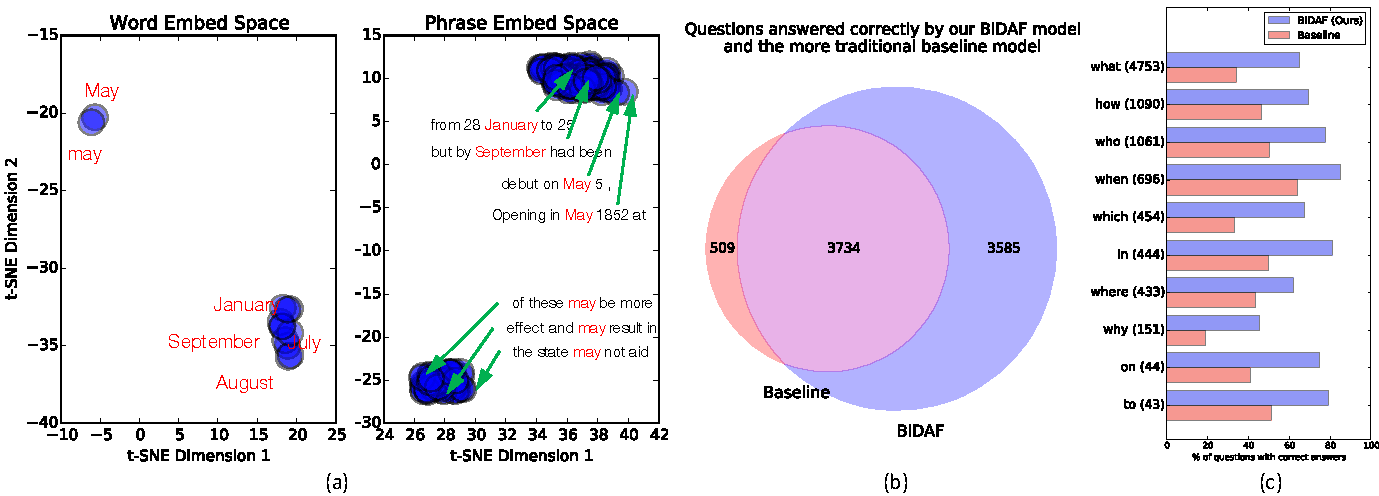
\includegraphics[width=34pc]{figures/subfigure}
\caption{\small (a) t-SNE visualizations of the \textit{months} names embedded in the two feature spaces. The contextual embedding layer is able to distinguish the two usages of the word \textit{May} using context from the surrounding text. (b) Venn diagram of the questions answered correctly by our model and the \textit{more traditional} baseline~\citep{rajpurkar2016squad}. (c) Correctly answered questions broken down by the 10 most frequent first words in the question.}
\label{fig:tsne}
\end{figure}

\begin{figure}[]
\centering
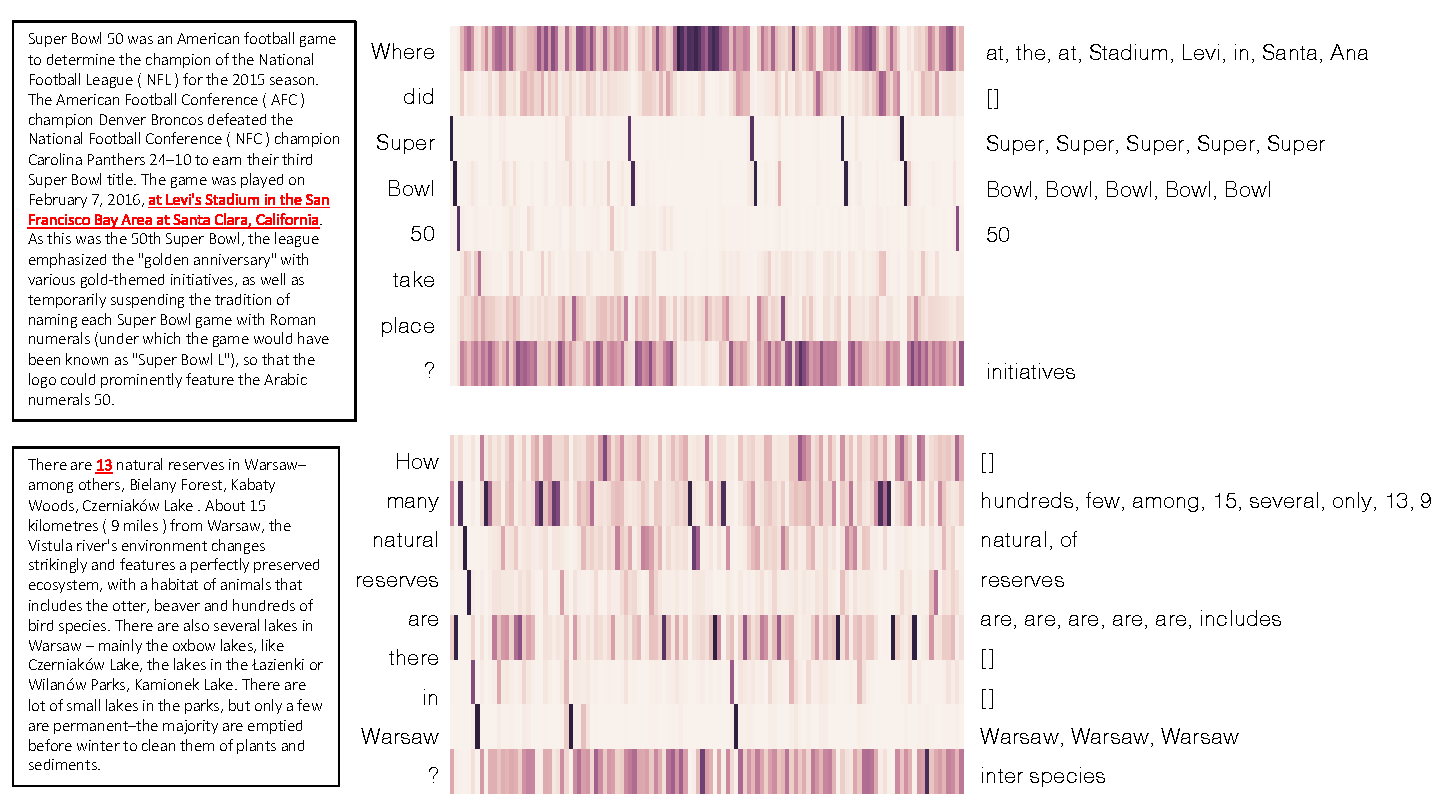
\includegraphics[width=30pc]{figures/attention_weights_viz_2}
\caption{\small Attention matrices for question-context tuples. The left palette shows the context paragraph (correct answer in red and underlined), the middle palette shows the attention matrix (each row is a question word, each column is a context word), and the right palette shows the top attention points for each question word, above a threshold.}
\label{fig:viz_attention}
\end{figure}

We also visualize these two feature spaces using t-SNE in Figure~\ref{fig:tsne}. t-SNE is performed on a large fraction of dev data but we only plot data points corresponding to the months of the year. 
An interesting pattern emerges in the Word space, where \textit{May} is separated from the rest of the months because \textit{May} has multiple meanings in the English language. 
The contextual embedding layer uses contextual cues from surrounding words and is able to separate the usages of the word \textit{May}. Finally we visualize the attention matrices for some question-context tuples in the dev data in Figure~\ref{fig:viz_attention}. In the first example, \textit{Where} matches locations and in the second example, \textit{many} matches quantities and numerical symbols. Also, entities in the question typically attend to the same entities in the context, thus providing a feature for the model to localize possible answers.



\paragraph{Discussions.} We analyse the performance of our our model with a traditional language-feature-based baseline~\citep{rajpurkar2016squad}. Figure~\ref{fig:tsne}b shows a Venn diagram of the dev set questions correctly answered by the models. Our model is able to answer more than 86\% of the questions correctly answered by the baseline. The 14\% that are incorrectly answered does not have a clear pattern. 
This suggests that neural architectures are able to exploit much of the information captured by the language features. 
We also break this comparison down by the first words in the questions (Figure~\ref{fig:tsne}c). Our model outperforms the traditional baseline comfortably in every category.

\paragraph{Error Analysis.} We randomly select 50 incorrect questions (based on EM) and categorize them into 6 classes.
50\% of errors are due to the imprecise boundaries of the answers,
28\% involve syntactic complications and ambiguities,
14\% are paraphrase problems,
4\% require external knowledge,
2\% need multiple sentences to answer,
and 2\% are due to mistakes during tokenization.
See Appendix~\ref{sec:error} for the examples of the error modes.